\documentclass[twocolumn]{article}
\usepackage{calc}
\usepackage{ifthen}
\usepackage[margin=0.5in]{geometry}
\usepackage{amsmath,amsthm,amsfonts,amssymb}
\usepackage{amsfonts}
\usepackage{color,overpic}
\usepackage{hyperref}
\usepackage{array} 
\usepackage{amstext}
\usepackage{enumitem}
\usepackage{graphicx}
\usepackage{caption}
\usepackage{natbib}
\usepackage{framed}
\usepackage{epigraph}
\usepackage{float}
%\usepackage[]{algorithm2e}
\usepackage{algpseudocode} 
\usepackage{algorithmicx}

\newenvironment{Figure}
  {\par\medskip\noindent\minipage{\linewidth}}
  {\endminipage\par\medskip}
  
\numberwithin{equation}{section}


% Turn off header and footer
\pagestyle{empty}
\setlist[itemize]{leftmargin=*} % set itemise indentation to leftmargin
\setlist[enumerate]{leftmargin=*}



\title{Learning Machine}
\date{\vspace{-6ex}}

% -----------------------------------------------------------------------

\begin{document}
\maketitle



\section{Introduction}

	\subsection{Definition}
\begin{framed}
\textbf{Machine learning} explores the construction and study of algorithms that can learn from and make predictions on data. Such algorithms operate by building a model from example inputs in order to make data-driven predictions or decisions, rather than following strictly static program instructions.
\end{framed}

	\subsection{History and Development}
Machine learning has evolved from the study of pattern recognition and computational learning theory in Artificial Intelligence.

\epigraph{Field of study that gives computers the ability to learn without being explicitly programmed}{Arthur Samuel, 1959}

\epigraph{A computer program is said to learn from experience E with respect to some class of tasks T and performance measure P, if its performance at tasks in T, as measured by P, improves with experience E}{Tom M. Mitchell}

\epigraph{Can machines think?}{Alan Turing, \textit{Computing Machinery and Intelligence}}

	\subsection{Categorisation}
Based on the nature of the learning signal,
\begin{itemize}
	\item In \textbf{supervised learning}, the goal is to learn a general rule that maps inputs to outputs based on a training dataset (input and output). 
	\item With \textbf{unsupervised learning}, no labels are available and the goal is to find structure from input only.
	\item \textbf{Reinforcement learning}, aims to take actions in an dynamic environment so as to maximize some notion of cumulative reward (such as driving a vehicle).
\end{itemize}
 Among other small categories, \textbf{semi-supervised learning} is dealing with incomplete training dataset, \textbf{learning to learn} learns its own inductive bias based on previous experience and \textbf{developmental learning} generates its own sequences of learning situations to cumulatively acquire novel skills.
 
 
Another categorization arises when considering outputs:
\begin{itemize}
	\item In \textbf{classification} (supervised) and \textbf{clustering} (unsupervised), inputs are divided into classes
	\item \textbf{In regression} (supervised), the outputs are continuous rather than discrete.
	\item \textbf{Density estimation} finds the distribution of inputs in some space.
	\item \textbf{Dimensionality reduction} simplifies inputs by mapping them into a lower-dimensional space
\end{itemize}




















\newpage
\section{Tool}

	\subsection{Tree}
\begin{itemize}
	\item A \textbf{graph} is mathematical structures used to model pairwise relations (\textit{edge} or line) between objects (\textit{vertices} or nodes). The edges may be \textit{directed} or \textit{undirected} for symmetric or asymmetric relation.

	\item In \textit{graph theory}, a \textbf{tree} is an undirected graph in which any two vertices are connected by exactly one path.

	\item An \textbf{ordered tree} is a rooted tree (one vertex has been designated as the root) for which an ordering is specified for the children of each vertex.

	\item In \textit{computer science}, a \textbf{tree data structure} is an ordered tree which has a value associated to each node.
	
	\item A \textbf{decision tree} is a decision support tool that uses a tree-like graph of decisions and their possible consequences (leaf), including chance event outcomes, resource costs, and utility. 
\end{itemize}


\subsection{Bayes}
\begin{itemize}
	\item \textbf{Bayes' theorem} relates an updated probability $P(A|B)$ to its prior probability $P(A)$ in relation to an event $B$ and its relation to it $P(B | A)$
$$P(A|B) = \frac{P(B | A)\, P(A)}{P(B)}$$
	\item \textbf{Bayes' Rule} is an equivalent way to formulate Bayes' theorem but relating only a proportional relation.
	$$P(A|B) \propto P(A)P(B|A) $$
	\item \textbf{Statistical inference} is the process of deducing properties of an underlying distribution by analysis of data
	\item \textbf{Bayesian inference} is a method of inference in which Bayes' rule is used to update the probability for a hypothesis as evidence is acquired.
$$p(\theta \mid \mathbf{X}) = \frac{p(\mathbf{X} \mid \theta) p(\theta)}{p(\mathbf{X})} \propto p(\mathbf{X} \mid \theta) p(\theta)$$
	where:
	\begin{itemize}
		\item $\theta$, the parameter
		\item $\mathbf{X}$, a set of n observed data points
		\item $p(\theta)$, the prior distribution
		\item $p(\theta \mid \mathbf{X})$, posterior distribution
		\item $ p(\mathbf{X} \mid \theta)$, sampling distribution or likelihood
		\item $p(\mathbf{X}) = \int_{\theta} p(\mathbf{X} \mid \theta) p(\theta) \operatorname{d}\!\theta $, marginal likelihood
	\end{itemize}

\end{itemize}


\subsection{Other}
In geometry, a \textbf{hyperplane} is a subspace of one dimension less than its ambient space.











\newpage
\section{List of Algorithm}

	\subsection{Decision tree learning}
The goal is to create a model that predicts the value of a target variable based on several input variables. Each interior node corresponds to one of the input variables and each leaf represents a value of the target variable given the values of the input variables represented by the path from the root to the leaf.
\begin{figure}[H]
	\centering
    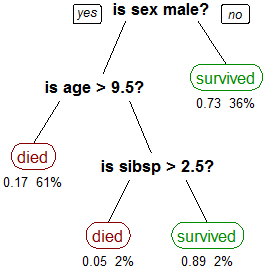
\includegraphics[width=.3\textwidth]{CART_tree_titanic_survivors.png}
    \caption{A tree showing survival of passengers on the Titanic ("sibsp" is the number of relative aboard). The figures under the leaves show the probability of survival and the percentage of observations in the leaf.}
\end{figure}



	\subsection{Support vector machines (SVMs)}
A SVM is a supervised non-probabilistic binary linear classifier which constructs a hyperplane able to separate the two categories.

Given some training data $\mathcal{D}$, a set of n points of the form
$$\mathcal{D} = \left\{ (\mathbf{x}_i, y_i)\mid\mathbf{x}_i \in \mathbb{R}^p,\, y_i \in \{-1,1\}\right\}_{i=1}^n$$
We want to find the maximum-margin hyperplane that divides the class. Any hyperplane can be written as the set of points $\mathbf{x}$ satisfying 
$$\mathbf{w}\cdot\mathbf{x} - b=0$$
Where $\mathbf{w}$ is the normal vector to the hyperplane and $\tfrac{b}{\|\mathbf{w}\|}$ is the hyperplane offset from the origin along $\mathbf{w}$.

\begin{figure}[H]
	\centering
	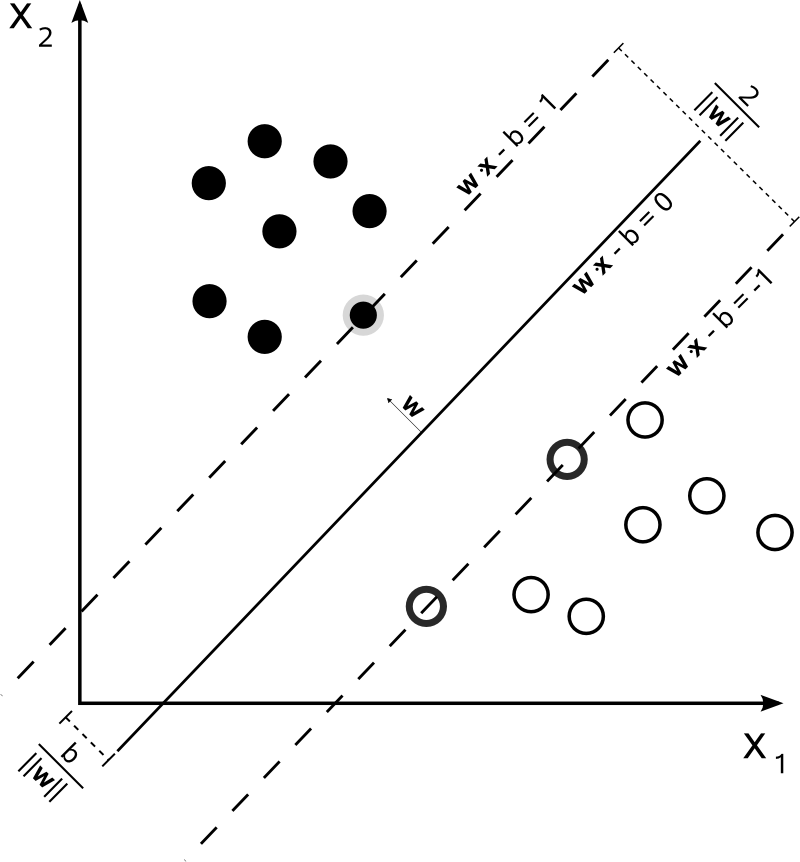
\includegraphics[width=.2\textwidth]{Svm_max_sep_hyperplane_with_margin.png}
\end{figure}
Graphicaly, the solution is fully determined by the nearest points which are called \textit{support vectors}.
Mathematically, we are looking at a function 
$$f(\mathbf{x})=\mathbf{w}\cdot\mathbf{x} - b = \left\{
  \begin{array}{lr}
    \ge 1 	& \text{class 1}\\
    0  		& \text{hyperplan} \\
    \le -1 	& \text{class 2}\\
    else    & \text{margin}
  \end{array}
\right.$$

The maximum-margin is achived when $\|\mathbf{w}\|$ is minimized, the optimization problem becomes
\begin{align*}
&\underset{\mathbf{w},b}{\operatorname{minimize}}& & \frac{1}{2}\|\mathbf{w}\|^2 \\
&\operatorname{subject\;to}
& &y_i(\mathbf{w}\cdot\mathbf{x}_i - b) \ge 1 
\end{align*}

For not linearly separable data, the hinge loss function penalazied data $\mathbf{x}_i$ on the wrong side of the hyperplan with
$$\max \left\{ 0,1-y_{i}( \mathbf{w}\cdot \mathbf{x}_i  -b) \right\}$$.

The optimization problem become 
\begin{align*}
&\underset{\mathbf{w},b}{\operatorname{minimize}}& &  \frac{1}{n} \sum_i \max \left\{ 0,1-y_{i}( \mathbf{w}\cdot \mathbf{x}_i  -b) \right\}  + \frac{1}{2} \lambda \|\mathbf{w}\|^2, \\
\end{align*}
where the parameter $\lambda$ determines the tradeoff between increasing the margin-size and ensuring that the $\mathbf{x}_i$ lie on the correct side of the margin.

A non-linear adaptation of SVM has been proposed by applying the kernel trick:  every dot product are replaced by a nonlinear kernel function.

The classical approach to solve this problem is see it as a quadratic programming problem (Lagrange multiplier for linearly separable data or Augmented Lagrangian method else). More modern algorithm solves this problem with gradient problem: sub-gradient descent (if there are many training examples) or coordinate descent (if the dimension of the feature space is high).

 	\subsection{Relevance vector machine (RVM)}
The RVM has an identical functional form to SVM, but provides probabilistic classification using Bayesian inference.
 	

	\subsection{Cluster analysis}
Clustering is the task of grouping objects such that objects in the same group are more both similar to each other and different to those in other groups.
Cluster Analysis can also be formulated as a multi-objective optimization.

		\subsubsection*{Hierarchical clustering}
This algorithm base similitude on a measure of distance (euclidian distance or others). Dendrogram is the best way to visualised the ``hierarchical'' aspect of this algorithm: the bottom axis is the distance where two cluster merge (or divide for top-down approch)
\begin{figure}[H]
	\centering
	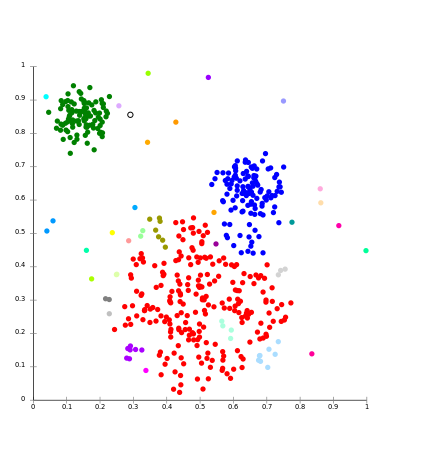
\includegraphics[width=.2\textwidth]{434px-SLINK-Gaussian-data.png}
	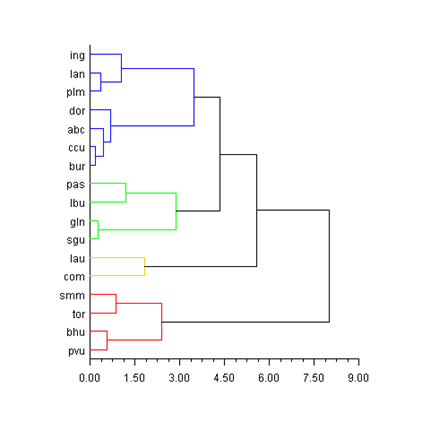
\includegraphics[width=.2\textwidth]{image271_28.png}
\end{figure}

		\subsubsection*{k-means algorithm}
K-means clustering gives a formal definition as an optimization problem: find the k cluster centers and assign the objects to the nearest cluster center.
 $$\underset{\mathbf{S}} {\operatorname{arg\,min}}  \sum_{i=1}^{k} \sum_{\mathbf x \in S_i} \left\| \mathbf x - \mathbf c_i \right\|^2 $$
with $\mathbf{x}$ being the observations point, $c_i$ the cluster center and $\mathbf{S}$ the k-set.
\begin{figure}[H]
	\centering
	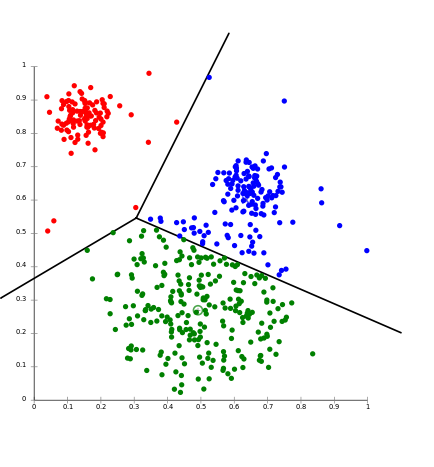
\includegraphics[width=.2\textwidth]{434px-KMeans-Gaussian-data.png}
\end{figure}

		\subsubsection*{Fuzzy}
In fuzzy clustering, data elements belong to a cluster according to a membership levels.

The widely used Fuzzy C-Means Algorithm (Bezdek 1981) is an adaptation of the k-mean algorithm where each element is compared to each center (not only one) and a partition matrix $w_i$ is introduced to describe the degree of membership.
 $$\underset{C} {\operatorname{arg\,min}}  \sum_{i=1}^{k} \sum_{j=1}^{n} w_{ij}^m \left\|\mathbf{x}_j - \mathbf{c}_i \right\|^2$$
 The fuzzifier $m$ determines the level of cluster fuzziness.
$$w_{ij} = \frac{1}{\sum_{u=1}^{k} \left(\frac{\left\|\mathbf{x}_j - \mathbf{c}_i \right\|}{\left\|\mathbf{x}_j - \mathbf{c}_u \right\|}\right)^{\frac{2}{m-1}}} \qquad \mathbf{c}_i = {{\sum_j {w_{ij}} ^ {m} x_j} \over {\sum_j {w_{ij}} ^ {m}}}$$
The algorithm converge by computing iteratly the weight and center.

	\subsection{Artificial neural network (ANNs)}
There is no single formal definition, however ANNS are capable of approximating a non-linear functions with a large number of inputs by mimicking biological neural networks.  Each nodes (neurons) consist of adaptive weights, parameters tuned by a learning algorithm. 
\begin{figure}[H]
	\centering
    $\vcenter{\hbox{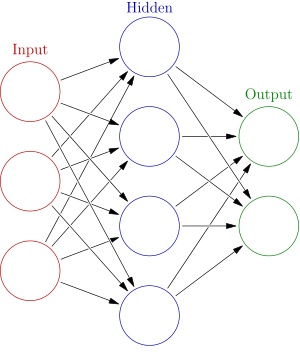
\includegraphics[width=.25\textwidth]{300px-Colored_neural_network.png}}}$
    $\vcenter{\hbox{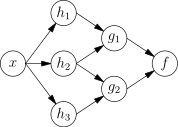
\includegraphics[width=.2\textwidth]{178px-Ann_dependency_(graph).png}}}$
\end{figure}	

		\subsubsection{Neurons Model}
\begin{itemize}
\item Linear neurons: output is a weighted some of the imput plus a bais 
$$z(x) = \sum_i w_i x_i + b$$
\item Binary threshold neurons: output is a step function for the weighted input exeeding a threshold $b$. 
$$y(x) = 1 \text{ if } z(x)>b \text{ else }0$$
\item Rectified Linear Neurons: combine a linear outpout with a threshold (low pass or high pass filter)
\item Sigmoid neurons: real-value output of a smooth and bounded function (eg: logistic function). Their nice derivative make learning easy.
$$ y(x) =\frac{1}{1+e^{-z}}$$
\item Stochastic binary neurons
Transform linear neurons or sigmoid neurons as a stocastic process:
$$P(s=1)=y(x)$$ 
\end{itemize}

		\subsubsection{Neural Network Architecture}
\begin{itemize}
\item Feed-forward neural networks: organized by layers: input layer -> hidden layers -> output layer
\item Recurrent neural networks: have cycles in their connection graph, difficult to train but much powerfull
\item Symmetricall connected networks are recurrent network with weight equal in both direction. much easier to analyze. They are called Hopfield nets if no hidden unit are present and “Boltzmann machines” otherwise.
\end{itemize}

		\subsubsection{Perceptron}
\textit{supervised learning, binary, linear classifiers}

	\subsection{Bayesian networks}
	\subsection{Genetic algorithms}
	\subsection{Bootstrap}
	\subsection{ANOVA}
	\subsection{Logistic regression}
	\subsection{k-nearest neighbor}



\bibliographystyle{apalike}
\bibliography{citations}	
	

\end{document}
